\newcommand{\svrname}{Mr Matthew Ireland}
\newcommand{\jkfside}{oneside}
\newcommand{\jkfhanded}{right}

\newcommand{\studentname}{Harry Langford}
\newcommand{\studentemail}{hjel2@cam.ac.uk}

\documentclass[10pt,\jkfside,a4paper]{article}

\newcommand{\svcourse}{CST Part IA: Software Engineering and Security}
\newcommand{\svnumber}{1}
\newcommand{\svvenue}{Microsoft Teams}
\newcommand{\svdate}{2022-05-11}
\newcommand{\svtime}{15:00}
\newcommand{\svuploadkey}{CBd13xmL7PC1zqhNIoLdTiYUBnxZhzRAtJxv/ytRdM1r7qIfwMsxeVwM/pPcIo8l}

\newcommand{\svrname}{Dr Sam Ainsworth}
\newcommand{\jkfside}{oneside}
\newcommand{\jkfhanded}{yes}

\newcommand{\studentname}{Harry Langford}
\newcommand{\studentemail}{hjel2@cam.ac.uk}

% DO NOT add \usepackage commands here.  Place any custom commands
% into your SV work files.  Anything in the template directory is
% likely to be overwritten!

\usepackage{fancyhdr}

\usepackage{lastpage}       % ``n of m'' page numbering
\usepackage{lscape}         % Makes landscape easier

\usepackage{verbatim}       % Verbatim blocks
\usepackage{listings}       % Source code listings
\usepackage{epsfig}         % Embed encapsulated postscript
\usepackage{array}          % Array environment
\usepackage{qrcode}         % QR codes
\usepackage{enumitem}       % Required by Tom Johnson's exam question header

\usepackage{hhline}         % Horizontal lines in tables
\usepackage{siunitx}        % Correct spacing of units
\usepackage{amsmath}        % American Mathematical Society
\usepackage{amssymb}        % Maths symbols
\usepackage{amsthm}         % Theorems

\usepackage{ifthen}         % Conditional processing in tex

\usepackage[top=3cm,
            bottom=3cm,
            inner=2cm,
            outer=5cm]{geometry}

% PDF metadata + URL formatting
\usepackage[
            pdfauthor={\studentname},
            pdftitle={\svcourse, SV \svnumber},
            pdfsubject={},
            pdfkeywords={9d2547b00aba40b58fa0378774f72ee6},
            pdfproducer={},
            pdfcreator={},
            hidelinks]{hyperref}


% DO NOT add \usepackage commands here.  Place any custom commands
% into your SV work files.  Anything in the template directory is
% likely to be overwritten!

\usepackage{fancyhdr}

\usepackage{lastpage}       % ``n of m'' page numbering
\usepackage{lscape}         % Makes landscape easier

\usepackage{verbatim}       % Verbatim blocks
\usepackage{listings}       % Source code listings
\usepackage{graphicx}
\usepackage{float}
\usepackage{epsfig}         % Embed encapsulated postscript
\usepackage{array}          % Array environment
\usepackage{qrcode}         % QR codes
\usepackage{enumitem}       % Required by Tom Johnson's exam question header

\usepackage{hhline}         % Horizontal lines in tables
\usepackage{siunitx}        % Correct spacing of units
\usepackage{amsmath}        % American Mathematical Society
\usepackage{amssymb}        % Maths symbols
\usepackage{amsthm}         % Theorems

\usepackage{ifthen}         % Conditional processing in tex

\usepackage[top=3cm,
            bottom=3cm,
            inner=2cm,
            outer=5cm]{geometry}

% PDF metadata + URL formatting
\usepackage[
            pdfauthor={\studentname},
            pdftitle={\svcourse, SV \svnumber},
            pdfsubject={},
            pdfkeywords={9d2547b00aba40b58fa0378774f72ee6},
            pdfproducer={},
            pdfcreator={},
            hidelinks]{hyperref}

\renewcommand{\headrulewidth}{0.4pt}
\renewcommand{\footrulewidth}{0.4pt}
\fancyheadoffset[LO,LE,RO,RE]{0pt}
\fancyfootoffset[LO,LE,RO,RE]{0pt}
\pagestyle{fancy}
\fancyhead{}
\fancyhead[LO,RE]{{\bfseries \studentname}\\\studentemail}
\fancyhead[RO,LE]{{\bfseries \svcourse, SV~\svnumber}\\\svdate\ \svtime, \svvenue}
\fancyfoot{}
\fancyfoot[LO,RE]{For: \svrname}
\fancyfoot[RO,LE]{\today\hspace{1cm}\thepage\ / \pageref{LastPage}}
\fancyfoot[C]{\qrcode[height=0.8cm]{\svuploadkey}}
\setlength{\headheight}{22.55pt}


\ifthenelse{\equal{\jkfside}{oneside}}{

 \ifthenelse{\equal{\jkfhanded}{left}}{
  % 1. Left-handed marker, one-sided printing or e-marking, use oneside and...
  \evensidemargin=\oddsidemargin
  \oddsidemargin=73pt
  \setlength{\marginparwidth}{111pt}
  \setlength{\marginparsep}{-\marginparsep}
  \addtolength{\marginparsep}{-\textwidth}
  \addtolength{\marginparsep}{-\marginparwidth}
 }{
  % 2. Right-handed marker, one-sided printing or e-marking, use oneside.
  \setlength{\marginparwidth}{111pt}
 }

}{
 % 3. Alternating margins, two-sided printing, use twoside.
}


\setlength{\parindent}{0em}
\addtolength{\parskip}{1ex}

% Exam question headings, labels and sensible layout (courtesy of Tom Johnson)
\setlist{parsep=\parskip, listparindent=\parindent}
\newcommand{\examhead}[3]{\section{#1 Paper #2 Question #3}}
\newenvironment{examquestion}[3]{
\examhead{#1}{#2}{#3}\setlist[enumerate, 1]{label=(\alph*)}\setlist[enumerate, 2]{label=(\roman*)}
\marginpar{\href{https://www.cl.cam.ac.uk/teaching/exams/pastpapers/y#1p#2q#3.pdf}{\qrcode{https://www.cl.cam.ac.uk/teaching/exams/pastpapers/y#1p#2q#3.pdf}}}
\marginpar{\footnotesize \href{https://www.cl.cam.ac.uk/teaching/exams/pastpapers/y#1p#2q#3.pdf}{https://www.cl.cam.ac.uk/\\teaching/exams/pastpapers/\\y#1p#2q#3.pdf}}
}{}


\usepackage{graphicx}
\graphicspath{ {./images/} }
\usepackage{enumitem}
\usepackage{tikz-timing}
\usepackage{multirow}
\usepackage{multicol}

\begin{document}

\begin{enumerate}
\item Show (using appropriate examples and schematic diagrams) how ROMs, 
PALs PLAs and FPGAs can be used to implement combinatorial logical functions. 
What are their relative advantages and disadvantages?

\begin{enumerate}
\item The literals in the combinatorical logic are used to address ROM. This reads the 
value which is writen there. So you can program the ROM with combinatorical and 
it will return it when addressed.

Using ROM to implemnet combinatorical logic ensures that the logical circuit is not 
changed -- and it does also not have to be hardwired.\\
So the same circuit can be reused without reprogramming even after power loss.

Unfortunately, using ROM for combinatorical logic means accessing memory -- which is slow.\\
And ROM wastes a lot of memory if the expression is sparse.
Since ROM cannot be edited, the logical expression is also fixed -- which is not ideal.

IE to implement the logical expression $f = ABC + \bar A\bar C + \bar B\bar C$ the 
ROM would store:

\begin{tabular}{|c|c|}
\hline
Address & Data\\
\hline
000 & 1\\
001 & 0\\
010 & 1\\
011 & 0\\
100 & 1\\
101 & 0\\
110 & 0\\
111 & 1\\
\hline
\end{tabular}

So using the literals to address the memory and returning the value would implement the 
combinatorical logic. ie a=0, b=0, c=0 would go to memory address 000 and read f=1.

\item PALs can be programmed in the AND plane -- and then the terms generated in the and 
plane are OR'd together in an immutable OR plane. For every output which the term is included 
in, it must be generated again. This means that PALs are innefficient if they have to 
generate many functions containing the same terms. However, since only the AND plane is 
programmable, they are fast, simple -- and the combinatorical expressions are not fixed.

In the diagram below:

\begin{center}
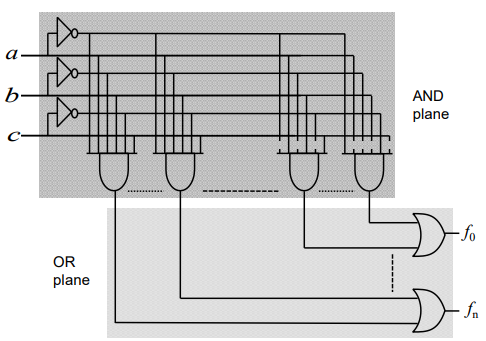
\includegraphics[width=0.5\textwidth]{1pal}
\\{\scriptsize Image from page 10 of the \href{https://www.cl.cam.ac.uk/teaching/2122/DigElec/slides/comb_beyond_20_1.pdf}{Digital Electronics Lecture Notes}}
\end{center}

The wires in the AND plane can be turned ``off''. This means that the expression represented 
by each AND gate can be changed and so different combinatorical expressions can be represented.
 However, the OR plane cannot be changed.\\
IE to represent $f_0 = ABC + \bar A\bar C$, we would turn off wires so that the circuit looked 
like this.

\begin{center}
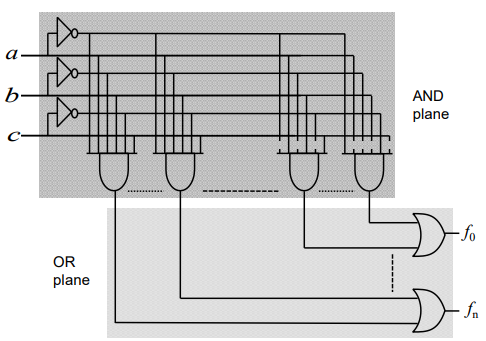
\includegraphics[width=0.5\textwidth]{1pal2}
\\{\scriptsize Modified version of an image on page 10 of the \href{https://www.cl.cam.ac.uk/teaching/2122/DigElec/slides/comb_beyond_20_1.pdf}{Digital Electronics Lecture Notes}}
\end{center}

\item PLAs can be programmed in both the AND and OR planes. This means that they are programmable, and 
so the logical expression they represent can be programmed. They can also re-use terms in other expressions
This makes them very efficient. However, since both the AND and OR planes are programmable, PLA's are 
very complicated and expensive.

To represent a logical expression using a PLA, you turn off wires in the AND plane so that the terms you 
want to OR together are generated. You then turn off the appropriate wires in the OR plane so that the 
terms all go into the same function.

IE if you wanted to generate the logical expression $f_0 = ABC + \bar A\bar C$ 
and also wanted to generate the logical expression $f_1 = ABC + \bar B\bar C$ you would use the PLA as 
shown below. This would allow you to reuse the $ABC$ term without having to re-generate it.

\begin{center}
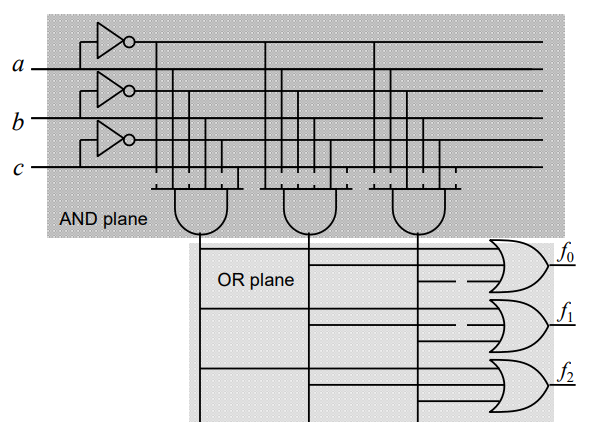
\includegraphics[width=0.5\textwidth]{1pla2}
\\{\scriptsize Modified version of an image on page 9 of the \href{https://www.cl.cam.ac.uk/teaching/2122/DigElec/slides/comb_beyond_20_1.pdf}{Digital Electronics Lecture Notes}}
\end{center}

\item FPGAs are arrays of ``Configurable Logic Blocks'' (CBS's). Each CLB contains a lookup table (made of SRAM), the ouputs of 
which are processed with logical expressions and then passed through multiplexers and SR latches (so that you can select which 
expression to pass on -- and to make the CLB's synchronous).
FPGA's contain lots (often hundreds) of CLB's. This means they are essentially large arrays of lookup tables and complex logic.
The expressions in CLB's are writen in SRAM -- this means that when power is lost, the expression vanishes. So it must be re-written 
every time the power is turned on. Often the data for this is stored in EEPROM, however sometimes it can just be written 
from the computer itself.

FPGA's can represent incredibly complicated expressions, they can also be reprogrammed. FPGA's also often have common logical 
expressions pre-programmed into them. For small/mid sized projects, FPGA's are often cheaper than alternatives since they are 
off-the-shelf and do not have to be custom built. However, FPGA's are expensive and so for large projects it's often cheaper 
to make the logical circuit specifically. FPGA's do use non-volatile memory and so have to be re-written after the power is 
turned off. This means that the logical expression must be stored separately. FPGA's can also be memory innefficient if the 
expression is very sparse. FPGA's are designed for incredibly complicated logical expressions and so are unsuitable for most 
applications (overly-powerful).

\begin{center}
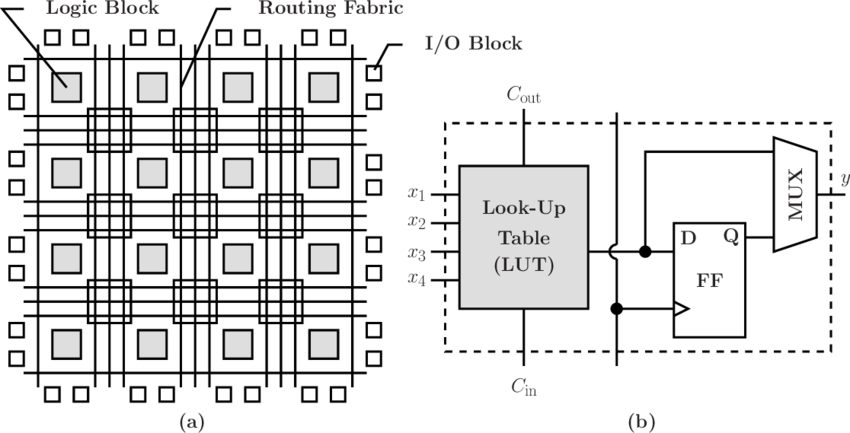
\includegraphics[width=0.5\textwidth]{1fpga}
\\{\scriptsize Image from \href{https://www.researchgate.net/figure/a-Sketch-of-the-FPGA-architecture-b-diagram-of-a-simple-logic-block-FF-flip-flop_fig7_276378036}{ResearchGate}}
\end{center}

To express a combinatorical logical function in a FPGA, you must split it up, then load parts of the expression into each CLB.
Then to evaluate the function with a given set of inputs, subsets of the inputs are passed into the CLB's, they then lookup the 
result in a lookup table and return them. Which outputs are output is determined by multiplexers. This is usually dependent on 
other inputs which that specific CLB was not passed.

\end{enumerate}

\item
\begin{enumerate}
\item How might one use an SR latch to debounce a SPDT switch? Draw timing diagrams to
illustrate your answer.

When turned on, a SPDT switch will change which output is set to 1. So at any one time, 
one output from an SPDT switch will always be 1 and another will always be 0. However, 
when pressed, the switch may ``flicker''. To mitigate this, we can attach the two outputs 
to a RS latch (as the input variables R and S, and then take $Q$ and $\overline Q$ as 
the new outputs.

This means that when the input flickers, and there are states where both outputs are off, 
$Q$ and $\overline Q$ will hold their previous values, hence debouncing the switch.

\begin{center}
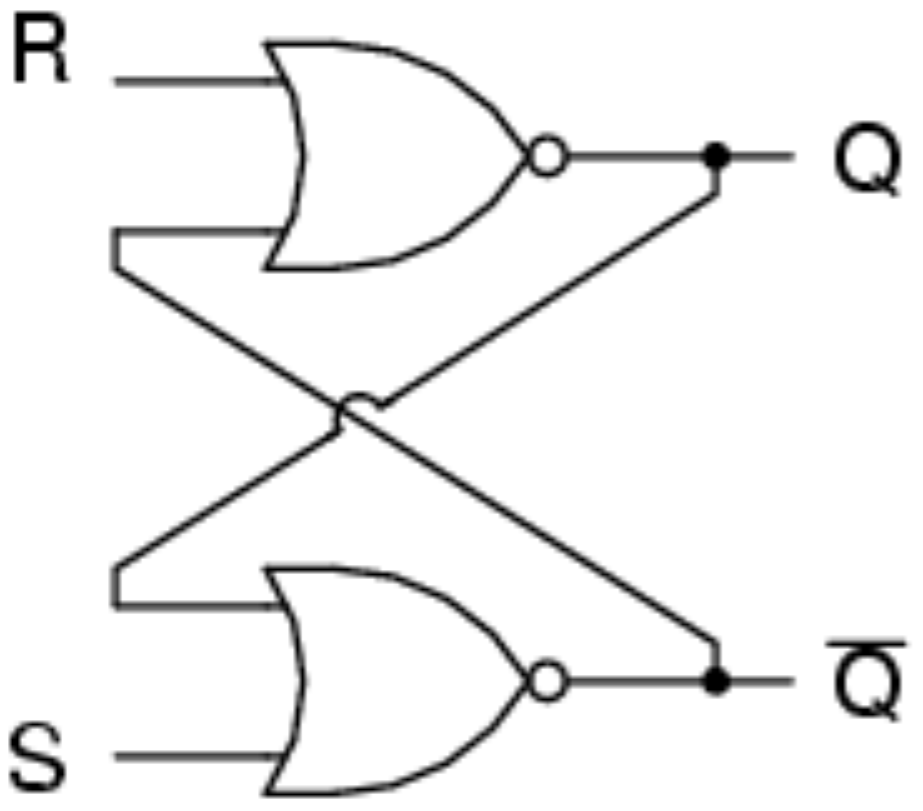
\includegraphics[width=0.3\textwidth]{2ars}
\end{center}

Take the timing diagram where R and S are the inputs from the SPDT switch.

Changing R from 1 to 0:

\begin{center}
{\huge
\begin{tikztimingtable}
$R$ & LLhlhlhlHHHHHHHHH \\
$S$ & HHHHHHHHhlhlhlLLL \\
$Q$ & LLHHHHHHHHHHHHHHH \\
$\overline Q$ & HHLLLLLLLLLLLLLLL \\
\end{tikztimingtable}
}
\end{center}

Changing S from 1 to 0:

\begin{center}
{\huge
\begin{tikztimingtable}
$R$ & HHHHHHHHhlhlhlLLL \\
$S$ & LLhlhlhlHHHHHHHHH \\
$Q$ & HHLLLLLLLLLLLLLLL \\
$\overline Q$ & LLHHHHHHHHHHHHHHH \\
\end{tikztimingtable}
}
\end{center}

As shown, the outputs from $Q$ and $\overline Q$ are equivalent but stable versions to 
the ouputs from the switch.
And so the RS Latch has been used to debounce the SPDT switch.

\item Suppose a NOR gate has a propagation delay equal to $\tau$. Further suppose that a particular
SR latch is in state Q = 1, and a clean pulse of length t appears on the R input in order
to reset the latch to state Q = 0. What is the minimum possible t, expressed in terms of
$\tau$, in order for the intended state change to be effected? Support your answer with timing
diagrams.

\begin{center}
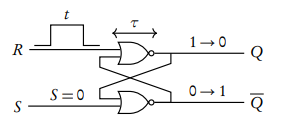
\includegraphics{2b}
\end{center}

The shortest pulse which will effect the change will have to be long enough to change both $Q$ and 
$\overline Q$. If a time $t = 0$ R pulses to 1, then at time $\tau$ the signal change will have 
propogated through the NOR gate and $Q$ will change to 0. At this point, $\overline Q$ will still be 
0 and so the circuit is \textbf{not} in a valid state. The signal must propogate throuth the bottom 
NOR gate to change $\overline Q$ to 1. This takes a further $\tau$. So at $t = 2 \tau$ the circuit 
will have completed the state change. So the total time is $2 \tau$.

If the pulse is turned off before this time; $Q$ will change back to 1.

So the minimum t which will cause the intended state change to be effected is 2$\tau$.

If the pulse lasts less than $2 \tau$ (in this case $\tau$)
Then the circuit will enter an illegal state.

{\Huge
\begin{tikztimingtable}
$R$ & LHHLLLLL \\
$Q$ & HHHLLHH \\
$\overline Q$ & LLLLLHH \\
\end{tikztimingtable}
}

If the pulse lasts $2 \tau$ or more then the state change will be effected properly.

{\Huge
\begin{tikztimingtable}
$R$ & LHHHHLLL \\
$Q$ & HHHLLLLL \\
$\overline Q$ & LLLLLHHH \\
\end{tikztimingtable}
}

\end{enumerate}

\item A machine has the state diagram shown below, where N and D are the two inputs and $N = D = 1$
cannot occur. The state assignment is $S_0 = [00]$, $S_1 = [01]$, $S_2 = [10]$ and $S_3 = [11]$, where the
machine starts in state $S_0$ and finishes in state $S_3$. Note that the state = $[Q_1Q_0]$ where $Q_n$ is the 
output of flip-flop n.

\begin{center}
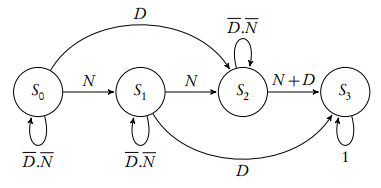
\includegraphics{3x}
\end{center}

\begin{enumerate}

\item{Write down the state transition table for this machine.}

\begin{center}
\begin{tabular}{|c|c|c|c|}
\hline
Current State & D & N & Next State\\
\hline
$S_0$ & 1 & 0 & $S_2$\\
$S_0$ & 0 & 1 & $S_1$\\
$S_0$ & 0 & 0 & $S_0$\\
$S_1$ & 1 & 0 & $S_3$\\
$S_1$ & 0 & 1 & $S_2$\\
$S_1$ & 0 & 0 & $S_1$\\
$S_2$ & 1 & 1 & $S_3$\\
$S_2$ & 1 & 0 & $S_3$\\
$S_2$ & 0 & 1 & $S_3$\\
$S_2$ & 0 & 0 & $S_2$\\
$S_3$ & 1 & 1 & $S_3$\\
$S_3$ & 1 & 0 & $S_3$\\
$S_3$ & 0 & 1 & $S_3$\\
$S_3$ & 0 & 0 & $S_3$\\
\hline
\end{tabular}
\end{center}

\item{Assuming the use of J-K flip-flops for the state registers, write down the modified state 
transition table and determine the minimised Boolean expressions for the next state functions.}

With $S_0$ as 00, $S_1$ as 01, $S_2$ as 10 and $S_3$ as 11:

\begin{center}
\begin{tabular}{|c|c|c|c|}
\hline
$Q_1Q_0$ & D & N & $Q_1Q_0$\\
\hline
00 & 1 & 0 & 10\\
00 & 0 & 1 & 01\\
00 & 0 & 0 & 00\\
01 & 1 & 0 & 11\\
01 & 0 & 1 & 10\\
01 & 0 & 0 & 01\\
10 & 1 & 1 & 11\\
10 & 1 & 0 & 11\\
10 & 0 & 1 & 11\\
10 & 0 & 0 & 10\\
11 & 1 & 1 & 11\\
11 & 1 & 0 & 11\\
11 & 0 & 1 & 11\\
11 & 0 & 0 & 11\\
\hline
\end{tabular}
\end{center}

$Q_1$:

\begin{center}
\begin{tabular}{|c|c|c|c|c|c|} 
\hline
& & \multicolumn{4}{c|}{$Q_1Q_0$} \\
\hline
& & 00 & 01 & 11 & 10 \\ 
\hline
\multirow{4}{2em}{$DN$} 
& 00 & 0 & 0 & 1 & 1 \\
& 01 & 0 & 1 & 1 & 1 \\
& 11 & x & x & 1 & 1 \\
& 10 & 1 & 1 & 1 & 1 \\
\hline
\end{tabular}
\end{center}

So $Q_1 = Q_1 + N + DQ_0$.

$Q_0$:

\begin{center}
\begin{tabular}{|c|c|c|c|c|c|} 
\hline
& & \multicolumn{4}{c|}{$Q_iQ_j$} \\
\hline
& & 00 & 01 & 11 & 10 \\ 
\hline
\multirow{4}{2em}{$DN$} 
& 00 & 0 & 1 & 1 & 0 \\
& 01 & 1 & 0 & 1 & 1 \\
& 11 & x & x & 1 & 1 \\
& 10 & 0 & 1 & 1 & 1 \\
\hline
\end{tabular}
\end{center}

So $Q_0 = Q_1\overline N + Q_1N + \overline Q_0N + \overline Q_1D$

\end{enumerate}

\item{Eliminate the redundant states from the following state table using the Row Matching approach.}

Row matching allows us to merge two rows into one if the next states and outputs are identical.

\begin{tabular}{c|c c|c c}
Current State & \multicolumn{2}{|c|}{Next State} & \multicolumn{2}{c}{Output($Z$)}\\
  & $X=0$ & $X=1$ & $X=0$ & $X=1$\\
\hline
A & A & B & 0 & 0\\
B & C & D & 0 & 0\\
C & A & D & 0 & 0\\
D & E & F & 0 & 1\\
E & A & F & 0 & 1\\
F & G & F & 0 & 1\\
G & A & F & 0 & 1\\
\end{tabular}

By inspection: $E$ and $G$ are identical. Merging them yields the table below:

\begin{tabular}{c|c c|c c}
Current State & \multicolumn{2}{|c|}{Next State} & \multicolumn{2}{c}{Output($Z$)}\\
  & $X=0$ & $X=1$ & $X=0$ & $X=1$\\
\hline
A & A & B & 0 & 0\\
B & C & D & 0 & 0\\
C & A & D & 0 & 0\\
D & E & F & 0 & 1\\
E & A & F & 0 & 1\\
F & E & F & 0 & 1\\
\end{tabular}

Now $D$ and $F$ are identical. Merging them gives the table below:

\begin{tabular}{c|c c|c c}
Current State & \multicolumn{2}{|c|}{Next State} & \multicolumn{2}{c}{Output($Z$)}\\
  & $X=0$ & $X=1$ & $X=0$ & $X=1$\\
\hline
A & A & B & 0 & 0\\
B & C & D & 0 & 0\\
C & A & D & 0 & 0\\
D & E & D & 0 & 1\\
E & A & D & 0 & 1\\
\end{tabular}

No states in this table are identical. 
So the table cannot be reduced any further using Row Matching.

\item
\begin{examquestion}{2002}{2}{2}

\begin{enumerate}[label=(\alph*)]

\item{A 4-bit shift register constructed from edge-triggered D-type flip flops is shown
below. If, on successive rising edges of the clock signal CLK, the input takes
on the values 1, 0, 1, 0, 1, 1, 1, 0, what are the contents of the shift register after
each edge of the clock? You may assume that the register contains all zeroes
initially.}

\begin{center}
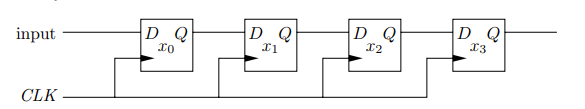
\includegraphics{5a}
\end{center}

\begin{center}
\begin{tabular}{c|c c c c}
input & $x_0$ & $x_1$ & $x_2$ & $x_3$\\
\hline
1 & 1 & 0 & 0 & 0\\
0 & 0 & 1 & 0 & 0\\
1 & 1 & 0 & 1 & 0\\
0 & 0 & 1 & 0 & 1\\
1 & 1 & 0 & 1 & 0\\
1 & 1 & 1 & 0 & 1\\
1 & 1 & 1 & 1 & 0\\
0 & 0 & 1 & 1 & 1\\
\end{tabular}
\end{center}

\item{Using a (possibly larger) shift register, show how one may detect a particular
pattern in the input shown. As an example, use the 8-bit pattern 0xF0. High order bits precede 
low-order bits in the input stream}

You would take the values $x_i$ as inputs to a block of combinational logic containing the pattern 
you wished to check for. f would then return 1 if the inputs matched that pattern.

\begin{center}
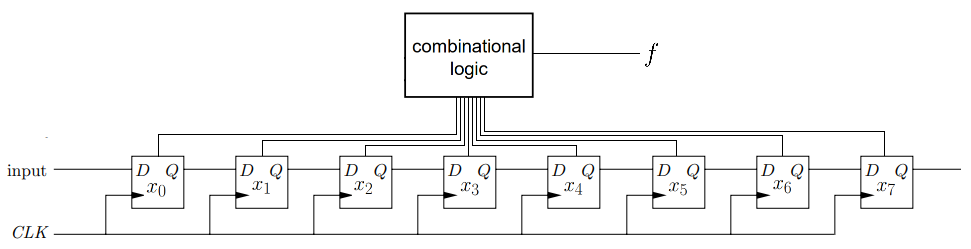
\includegraphics[width=0.8\textwidth]{5shift8}
\end{center}

For the example $0xF0$, the combinational logic expression would be

$f = \bar x_0\bar x_1 \bar x_2\bar x_3\bar x_4\bar x_5\bar x_6\bar x_7$.

\item{The input stream is framed by a one byte frame pattern (0xF0) every 256 bytes.
However, the frame pattern may also appear at an arbitrary position in the
input stream.\\
It is required to design a framing circuit which generates two outputs:
framelock, which is asserted when the circuit ``believes'' it has determined
where the frame boundaries are, and frame pointer, which is asserted on
the clock edge immediately after the frame marker is detected. The circuit
“believes” itself to be locked to the frame structure when two successive frame
patterns have been found 256 bytes (i.e. 2048 bits) apart. The circuit should
not respond to unaligned frame patterns while it believes itself to be in lock
or if, once in lock, it has missed fewer than two expected frame patterns.\\
Draw a state diagram for the finite state control of the circuit. You may assume
the existence of an 11-bit resettable counter. You should consider the process
of assuming lock, maintaining lock and the accommodation of a single missed
framing pattern. State explicitly any additional assumptions you make.}

I'm not sure I fully understood this question, however have written a full 
explanation of how to implement a system which detects a first frame marker
 and then waits to match with a second frame marker 2048 bits after the first. 
 If it doesn't find it, it will then go back to the waiting state.
If it receives this it will set a RS latch indicating ``framelock'' to 1, and 
send a single pulse (the ``frame pointer'') then move to another state which outputs 
a continuous signal indicaign ``framelock''.

You'd implement an 8-bit shift register.

There would then be a block of combinational logic which would take the values in the 
shift register, the ``framelock'' bit as an input. It would display positive only 
when the framelock was, the values in the shift register matched the pattern.

If the combinational logic is 1 and the counter is not on, then the clock will start counting.
If the combinational logic is 1 and the clock is 2048, then a RS latch which outputs ``framelock''
 will be set to 1, and a single pulse indicating the ``frame pointer'' will be set to 1.
The combinational logic being positive would set a RS latch to 1 and make the counter 
start counting.
If the RS latch was already on, however it would not do this.
\newpage
The following is a state diagram of this:

$X$ means the pattern is matched

$Y$ means the counter is 2048

$S_1$ is the waiting state -- where the circuit is waiting for the first frame marker.

$S_2$ is the counting state -- where the circuit is counting 2048 bits and waiting for the second marker.

$S_3$ is when the ``frame pointer'' and ``framelock'' are both 1.

$S_4$ is where the circuit is locked -- ``framelock'' is 1..

\begin{center}
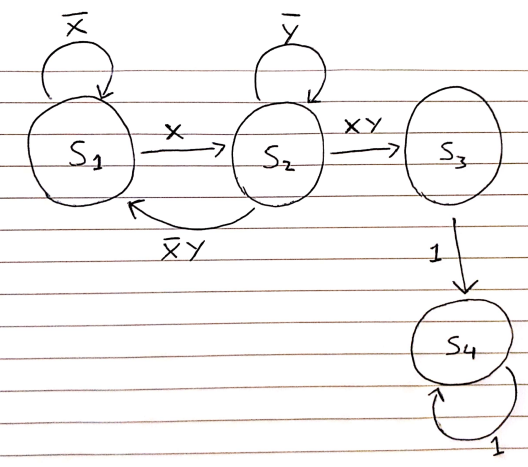
\includegraphics[width=0.8\textwidth]{5state}
\end{center}

\item{Outline the complexity in gates and flip flops for an implementation of the
framing circuit.}

You would need circuitry for the combinational logic, (a 8 input and gate or equivalent in 2-input and gates),
 two RS latches to hold the current state of the circuit. Other small pieces of logic to transition between 
 states.

\end{enumerate}
\end{examquestion}

\item The input to the first stage of a five-stage shift register is obtained from the 
exclusive-OR function of the outputs of the 3rd and 5th stages. Consider at the start 
that all 5 stages have a 1 output that shifts to the right on the application of each clock 
pulse. What is the output sequence expressed as a decimal number, taking the right 
(5th) stage as the least significant bit? After how many clock pulses does it repeat?
What happens if all 5 stages have 0 set on them at the start? 

In order to achieve the behaviour where you cycle through
every possible number (except 0), is it important that you connect together the outputs of the
$3^{rd}$ and $5^{th}$ stages, specifically? Would this work for any length of shift register (not just those
with 5 stages)?

The output sequence is 31.

It cycles through all possible integers (except 0).

It is 31 clock pulses before the sequence repeats.

If all 5 stages have 0 set on them at the start then the sequence remains at 0.

It is not important to connect together the outputs from of the $3^{rd}$ and $5^{th}$ stages specifically.
For example, cycling also works with the $2^{nd}$ and $5^{th}$ stage. It is however, essential that one of 
the bits is the \textbf{last} bit. But the other bit being the $3^{rd}$ bit in this case is coincidental.

This does not work for any length of shift register. Take for example a shift register of length 6. 
The $3^{rd}$ and $5^{th}$ bits cause it to cycle infinitely, never returning to $111111$. In order for 
a shift register of length 6 to return to $111111$, it would have to be in a state $111110$. However, 
when it is in this state; the output from the XOR of the $3^{rd}$ and $5^{th}$ bits is 0. So a shift 
register of length 6 will not return to $111111$ by XOR-ing together it's 3rd and 5th bits.

\end{enumerate}
\end{document}